
\section{\label{sec:CMS}Trigger System at the CMS Experiment}
The Compact Muon Solenoid (CMS) detector operates at the LHC\cite{collaboration2008cms}. Along with the ATLAS experiment it is one of the two general-purpose detectors in operation at the LHC used to study proton-proton (and lead-lead) collisions with a centre-of-mass energy of $13.6$TeV and at an instantaneous luminosity of up to $2 \cdot 10^{34} cm^{-2}s^{-1}$ in Run 3.
\par

At the Run 3 design luminosity a mean of around 50 inelastic collisions will occur in each bunch crossing with a frequency of around $40$MHz. Since the response and readout times of some detector elements may exceed the $25$ns spacing between bunch crossings the design and performance of the trigger is crucial to the physics data-taking operation.[citation?]


\subsection{The CMS Detector}

% At the centre of the CMS detector is a $13$m long, $3.8$T superconducting solenoid with a diameter of $6$m, that gives the experiment its name\cite{bayatian2006cms}. Inside the coil of the magnet the cylindrical structure of the detector is as follows: silicon pixel and strip trackers, a lead-tungstate scintillating-crystals electromagnetic calorimeter and a brass-scintillator sampling hadron calorimeter. The outermost layers of the detector, outside the solenoid, contain the muon system/detectors. There are 4 muon stations each consisting of several layers of aluminium drift tubes in the barrel and cathode strip chambers in the endcap region. In the forward regions of the detector the barrel calorimeter are complimented by further iron/quartz-fibre calorimeters increasing the pseudorapidity coverage.
% A more detailed description of the CMS detector, together with naming conventions, coordinate system definition and relevant kinematic variables can be found in \cite{cms_detector}. 


The central feature of the CMS apparatus is a superconducting solenoid of 6\unit{m} internal diameter, providing a magnetic field of 3.8\unit{T}. Within the solenoid volume are a silicon pixel and strip tracker, a lead tungstate crystal electromagnetic calorimeter (ECAL), and a brass and scintillator hadron calorimeter (HCAL), each composed of a barrel and two endcap sections. Forward calorimeters extend the pseudorapidity coverage provided by the barrel and endcap detectors. Muons are measured in gas-ionization detectors embedded in the steel flux-return yoke outside the solenoid. A more detailed description of the CMS detector, together with a definition of the coordinate system used and the relevant kinematic variables, can be found in Ref.~\cite{collaboration2008cms}. 
%Duplicated later?
% Events of interest are selected using a two-tiered trigger system. The first level (L1), composed of custom hardware processors, uses information from the calorimeters and muon detectors to select events at a rate of around 100 \unit{kHz} within a fixed latency of 4 \unit{\mu s} ~\cite{CMS:2020cmk}. The second level, known as the high-level trigger (HLT), consists of a farm of processors running a version of the full event reconstruction software optimized for fast processing, and reduces the event rate to around 1 \unit{kHz} before data storage~\cite{CMS:2016ngn}.




\subsection{The CMS Trigger}
As previously discussed the event rate at the LHC far exceeds the processing and storage capabilities of the four major experiments. 
Only a small fraction of the bunch crossings contain interactions of interest to the physics program of CMS. It is therefore the job of the CMS trigger system to separate the events to be saved amid the huge background event rate.
\par

The trigger system employed by the CMS collaboration reduces the event rate in two sequential steps of decision-making, the Level 1 and High Level Trigger.  


\subsubsection{L1 Trigger}
The first step in the trigger called Level 1 (L1) is characterized by its use of custom/bespoke hardware to drastically and rapidly reduce the event rate. Much of the L1 trigger logic is implemented in custom Application Specific Integrated Circuits (ASICs), Field Programmable Gate Arrays (FPGAs), Programmable Logic Devices (PLDs) and discrete logic such as memory Look-Up Tables (LUTs)\cite{cms2016cms,cms2020performance}.
\par

The initial L1 trigger decision occurs with a latency of $4 \mu$s and reduces the  rate from $40$MHz to a maximum of $100$kHz, limited by the detector readout. 
Crucially, the L1 hardware only has access to a coarse segmentation of data read-out from the calorimeters and the muon system as well as some correlation of information between these systems\cite{fontanesi2022cms}.


%maybe too long?
% As stated, the L1 trigger decision is made using simplified readout from the calorimeters (ECAL,HCAL,HF) and muon chambers (CSC, DT, RPC) that are called trigger primitives. All tracker information is not available to the L1 trigger. Trigger primitives are subsequently combined to form calorimetric towers and to link compatible muon hits together. These composite trigger primitives are then used to form the L1 trigger objects and the event achieves an L1 accept if the L1 trigger objects fulfill at least one of the pre-defined conditions of the L1 menu, as evaluated in the global trigger. The global trigger is the final part of the L1 trigger system and implements a menu of triggers/selection requirements on final L1 objects.
% See [ref] for a more detailed description of the working scheme of the TPs in L1.



\subsubsection{High Level Trigger}

The second step of the CMS trigger is the High Level Trigger (HLT). Implemented entirely in software running on a farm of commercial computing cores ($26,000$ in Run 3), called the Event Filter Farm (EVF), the HLT reduces the rate from the L1 output $100$kHz by a further factor 100 to $1$kHz with a maximum latency of $500$ms\cite{cms2023development,trocino2014cms,donato2018cms}.
\vspace{12pt}

The central aim of the HLT is to replicate as closely as possible the performance of algorithms and processing used in ``offline" analyses using the full detector resolution. Many ``streamlined" versions of offline reconstruction and analysis algorithms are utilized at this stage.
\par

% The HLT relies on the EVF to unpack the raw data into detector-specific data structures and to assemble complete event readouts from these partial fragments.
The flow of data in the HLT follows a \textit{path}-like structure of successive processing, reconstruction and selection algorithms. There are hundreds of HLT paths reconstructing and filtering based on different physics objectives. If an event is rejected by a filter then any subsequent reconstruction filtering modules for the path are cancelled.
The complexity, time requirements and physics sophistication of each step increases along the path. The aim of the algorithms is to both produce physics objects and select the events based on these objects. 
Those events that complete their processing path are stored locally on disk memory before being transferred to the CMS Tier-0 computing centre. Before transfer, the events are grouped into a set of non-exclusive streams including: primary physics, monitoring, calibration, parked and scouting\cite{thomas2019cms}.
\vspace{12pt}


The final output rate of the HLT is largely determined by the event size in terms of memory storage, as the limitation comes from the computing resources needed for downstream systems (CMS Tier-0) to process events. The data acquisition system can actually transfer $5-6$kHz. 


\subsubsection{Particle Flow}





\subsection{Upgrades}



\subsubsection{Run 3}

% In preparation for the current LHC Run 3 the CMS trigger underwent a series of improvements/optimisations that we shall presently discuss. 
The CMS physics program for Run 3 places a large focus on flavour physics, long-lived particles and Higgs sensitivity\cite{fontanesi2022cms,dordevic2022cms}, in light of this a number of sub-detectors and trigger algorithms were improved/replaced during LS2\cite{morovic2023cms}, some of which shall be presently discussed.
\vspace{12pt}

The HCAL sub-detector has received new on-detector electronics equipped with silicon photomultipliers (SiPMs) with triple the photon detection efficiency\cite{strobbe2017upgradecms} of the previous hybrid photodiodes. The ECAL sub-detector updated its L1 \textit{Spike Killer}\cite{daci2011cms} implementation, optimized the digitizer sum weights for Run 3 pile-up conditions and introduced a new double amplitude weights mechanism for further pileup suppression\cite{tishelman2022ecalcms}. The muon system Cathode Strip Chambers (CSCs) on-detector electronics were replaced with high speed optical links and more powerful processors. Additionally, a new gas electron multiplier (GEM) was installed covering the pseudo-rapidity region $1.6<|\eta|<2.4$\cite{battilana2019sissacms,colaleo2015cms}.
\vspace{12pt}

In Run 3 a demonstrative L1-scouting system has been tested\cite{morovic2023cms,ardino202340cms} with the aim of broadening the physics reach of CMS. The scouting stream retrieves L1 trigger data at the full LHC collision rate via specialized FPGA boards and saves the output for analysis, circumventing the HLT entirely. In the HLT all compute nodes are now equipped with two Nvidia T4 GPUs\cite{bocci2023cms} and for the first time approx. $40\%$ of CPU capacity now offloaded to these GPUs (initially only for pixel, ECAL and HCAL sub-detector reconstruction\cite{andre2019cms}.)
\vspace{12pt}

The tracking paradigm was significantly revised for Run 3 and is now performed using only a single global iteration, the Patatrack algorithm\cite{bocci2020heterogeneouscms,cms2018patatrack} in the HLT. Patatrack offers improved performance over the four-hit pixel tracking used for data taking in Run 2 while requiring fewer iterations and less CPU time. 
\vspace{12pt}

There have also been a substantial number of innovative online reconstruction algorithms developed for Run 3. These algorithms include, among many others, the discrimination of heavy flavour jets using DeepJet\cite{bols2020jetcms} and ParticleNet\cite{qu1902particlenetcms}. In addition to tracks, the DeepJet algorithm also
uses information from neutral and charged particle-flow jet constituents, whereas the ParticleNet algorithm represents jets as particle clouds in multiclass flavour classification. 
\par

A boosted decision tree classifier and neural network are employed in the search and seeding of muon reconstruction in the HLT\cite{cms2023development} with a $15\%$ reduction in CPU time. In Run 3 tau reconstruction the DeepTau\cite{cms2022identification} neural network was adapted from the offline reconstruction such that it matched HLT speed and performance requirements.

 


 % In fact, PF sees significant improvement with the tracks found by the Patatrack algorithm as input. . 


\subsubsection{Run 4 and Beyond}

In view of the HL-LHC, CMS is planning to entirely replace its trigger and data acquisition system and has a large upgrade program in place to facilitate the improvements required to take full advantage of the order of magnitude increase in luminosity. Several new sub-detectors are imagined in order to improve on current particle reconstruction and in order to manage the increased particle flux and pile-up conditions. 
\vspace{12pt}

The inner and outer tracker systems will undergo a full replacement with increased forward acceptance and more readout channels \cite{collaboration2017phasecms}. 
\par
A new MIP Timing Detector (MTD) will be installed between the tracker and calorimeter adding precise measurement of production time of MIP particles, at a resolution of around $30$ps\cite{cms2019mip}. 
\par
The endcap calorimeters will be replaced with hexagonally segmented high granularity calorimeters (HGCAL) capable of $3$ dimensional imaging of particle shower shape, including precision timing and energy measurement\cite{cms2017phase-hgcal,magnan2017hgcalcms,martelli2017cms,lobanov2020precisioncms}.
\par
The ECAL in the barrel region will receive new electronics capable of withstanding higher radiation while maintaining required readout, and will then return single crystal energies and timing to L1, instead of current $5\times 5$ cell summations\cite{cms2017phase-ecal}.
\par
The muon system's DTs and CSCs on-detector electronics will be replaced as well and improved GEM and RPC detectors will be installed in the inner ($\eta=2.4 - 2.8$) region and outer forward regions respectively\cite{cmsphase-muons,colaleo2015cms}. 
\vspace{12pt}



\begin{figure}[t!]
    \centering
    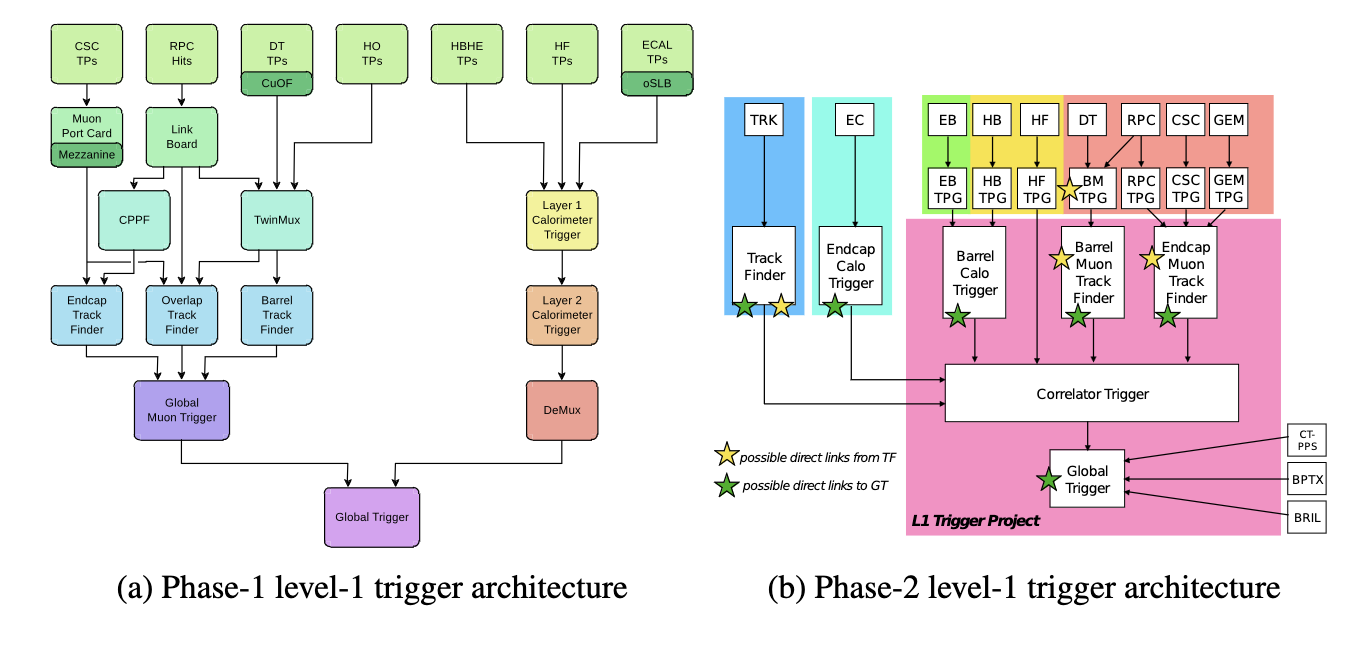
\includegraphics[width=0.7\linewidth]{images/cms/l1t-phase2.png}
    \caption{Overview of the Phase-1 (Run 2) and Phase-2 (Run 4) level-1 trigger architectures. In the former, inputs from the calorimeter and muon chamber are sent to the respective trigger subsystems, which are responsible for computing trigger objects. In the latter, three new systems are introduced: the endcap calorimeter trigger, responsible for processing data from HGCAL; the track finder, which reconstructs tracks in the tracker; the correlator trigger, which runs particle flow algorithms\cite{bologna2019overviewcms}.}
    \label{fig:cms-L1}
\end{figure}

In order to even maintain the current trigger performance in efficiency, resolution and background rejection the TDAQ system requires significant advancement. These performance improvements come jointly from the detector upgrades and their employment in reconstruction algorithms/trigger primitive decisions.
\par
In the upgraded L1 trigger\cite{bologna2019overviewcms} the maximum event rate is increased to $750$kHz from the previous $100$kHz with a new latency of $12.5${\textmu}s. L1 will now incorporate tracking inputs (for particles with $p_T$ exceeding a configurable threshold) in $|\eta|<2.4$. The track stubs will be filtered in an FPGA-based parallelized track-finding system. $3$ dimensional energy clusters from HGCAL will be included together with a full granularity readout of the barrel ECAL. The L1 trigger will have the capability to execute composite correlator trigger algorithms such as PF\cite{petrucciani2019particlecms} or Pile-Up-Per-Particle-Identification (PUPPI)\cite{kreis2018particlecms,bertolini2014puppi}.
\vspace{12pt}

The HLT in HL-LHC conditions will be required to manage a much higher event rate, more complex events and therefore a vast increase in computing requirements\cite{collaboration2021cmshlt}. The HLT will, as it does in Run 3, reduce the L1 event rate by a factor $100$; in the high-luminosity conditions this rate will be between $5$ and $7.5$kHz.
It is envisioned that $\sim 80\%$ of the computing workload will be ported to GPUs or other co-processors\cite{morovic2023cms}. The HLT will leverage the new HGCAL sub-detector and new tracker system, however these new sub-detectors are much more complex than their predecessors and the HLT will be required to have a throughput of $44$ Tb/s\cite{tomei2022hltcms}.






% \url{https://cds.cern.ch/record/2797771/files/CR2019_165.pdf}


